\documentclass{standalone}

\usepackage{tikz}
\usetikzlibrary{calc}

\begin{document}

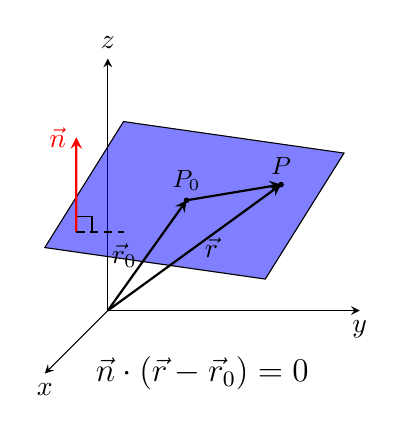
\begin{tikzpicture}[scale=0.8]

\coordinate (O)  at (0,0);
\coordinate (P1) at (-1,1);
\coordinate (P2) at (0.25,3);
\coordinate (P3) at (3.75,2.5);
\coordinate (P4) at (2.5,0.5);
\coordinate (N1) at (-0.5,1.25);
\coordinate (N2) at ($(N1)+(0,1.5)$);
\coordinate (Q1) at (1.25,1.75);
\coordinate (Q2) at ($(Q1)+(1.5,0.25)$);

\draw[-stealth] (O)--++(-1,-1) node[below] {$x$};
\draw[-stealth] (O)--++(4,0) node[below] {$y$};
\draw[-stealth] (O)--++(0,4) node[above] {$z$};

\filldraw[black, fill=blue, fill opacity=0.5] (P1)--(P2)--(P3)--(P4)--cycle;
\draw ($(N1)+(0.25,0)$)--++(0,0.25)--++(-0.25,0);
\draw[-stealth, red, thick] (N1)--(N2) node[left] {$\vec n$};
\draw[-stealth, thick] (O)--(Q1) node[midway, left] {$\vec r_0$};
\draw[-stealth, thick] (O)--(Q2) node[midway, right] {$\vec r$};
\draw[densely dashed, thick] (N1)--++(0.75,0);
\draw[-stealth, thick] (Q1)--(Q2);
\draw[fill=black] (Q1) circle (1pt) node[above] {\small$P_0$};
\draw[fill=black] (Q2) circle (1pt) node[above] {\small$P$};

\node at (1.5,-1) {\large$\vec n \cdot \left(\vec r - \vec r_0\right)=0$};

\end{tikzpicture}

\end{document}